\documentclass[border=3pt]{standalone}
% Preâmbulo compartilhado pelos diagramas TikZ da aula 13 (SLAM com EKF)
\usepackage[T1]{fontenc}
\usepackage[utf8]{inputenc}
\usepackage{lmodern}
\usepackage{amsmath}
\usepackage{xcolor}
\usepackage{tikz}
\usetikzlibrary{arrows.meta,angles,quotes,decorations.pathmorphing,decorations.pathreplacing,calc,
                positioning,shapes.geometric,shapes.misc,backgrounds,fit,
                math}

% Paleta (mesma dos SVGs originais)
\definecolor{dblue}{HTML}{2A5B8C}
\definecolor{dorange}{HTML}{B3541E}
\definecolor{dgreen}{HTML}{4A7C59}
\definecolor{dred}{HTML}{9C4B4B}
\definecolor{dcream}{HTML}{F4F1EA}
\definecolor{dshade}{HTML}{DDD7C9}

% Função gaussiana (não normalizada por padrão de escala visual)
\pgfmathdeclarefunction{gauss}{3}{%
  \pgfmathparse{1/(#3*sqrt(2*pi))*exp(-((#1-#2)^2)/(2*#3^2))}%
}

% Estilos comuns (prefixo d... para não colidir com chaves internas do pgf)
\tikzset{
  >={Stealth[length=2mm]},
  dguide/.style={gray!55, dashed, line width=0.4pt},
  daxis/.style={gray!60, line width=0.7pt, ->},
  dbody/.style={fill=black!3, draw=black!80, line width=1pt},
  dacc/.style={draw=dblue, line width=1pt},
  dlbl/.style={black!55, font=\small},
  dsub/.style={black!45, font=\footnotesize},
  dstate/.style={circle, draw=black!80, fill=dcream, line width=1pt,
                 minimum size=17mm, font=\large, inner sep=1pt},
  dobs/.style={circle, draw=black!80, fill=dshade, line width=1pt,
               minimum size=14mm, font=\large, inner sep=1pt},
  dbox/.style={rounded corners=2pt, draw=black!80, fill=dcream, line width=1pt,
               align=center, inner sep=6pt},
  dop/.style={circle, draw=black!80, fill=white, line width=1pt,
              minimum size=6mm, inner sep=0pt, font=\small},
  dtrans/.style={->, dblue, line width=1pt},
  dmeas/.style={->, dorange, line width=1pt},
  dcurve/.style={line width=1pt, dblue},
  dcurveb/.style={line width=1.4pt, dorange},
}

\begin{document}
\hyphenpenalty=10000 \exhyphenpenalty=10000 \tolerance=9999 \emergencystretch=3em
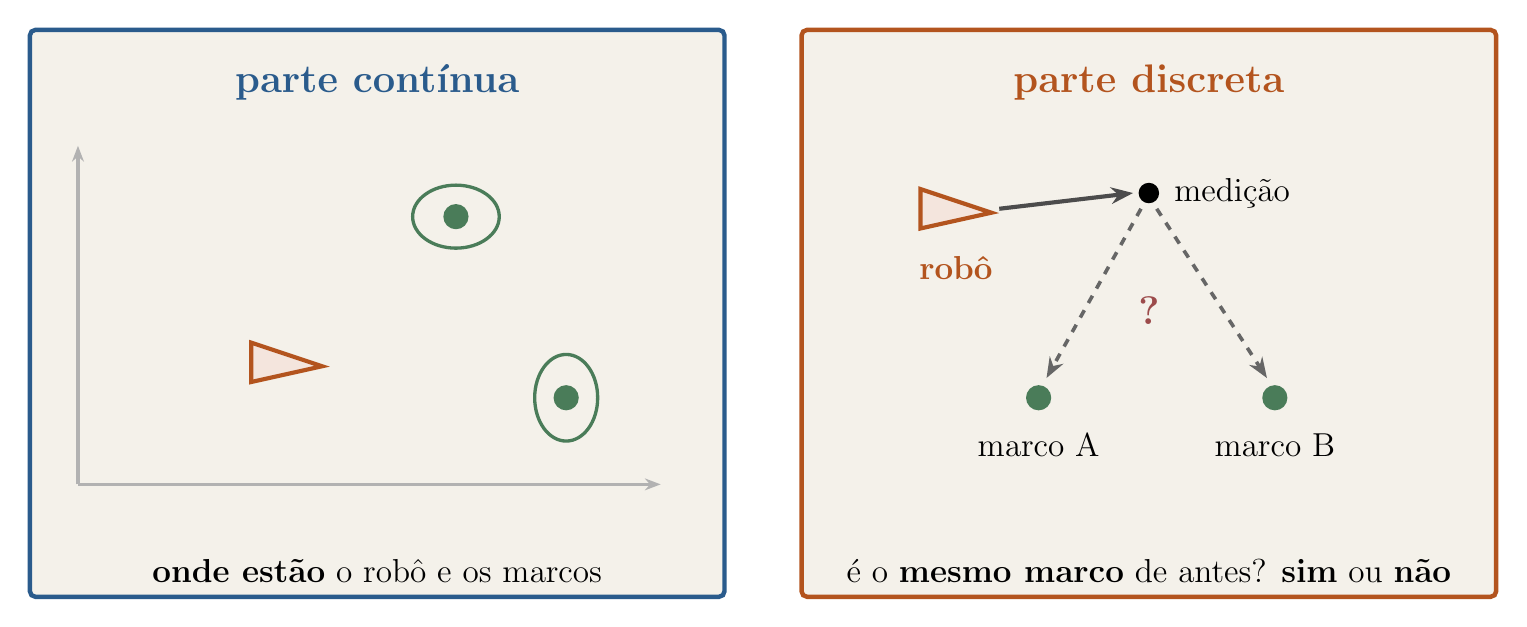
\begin{tikzpicture}[x=1cm,y=1cm]
\tikzset{c/.style={dbox, text width=8.4cm, minimum height=7.2cm, line width=1.6pt, font=\large, anchor=north}}
\node[c, draw=dblue] at (4.6,7.9) {};
\node[font=\Large\bfseries, dblue] at (4.6,7.2) {parte contínua};
\draw[daxis, line width=1.1pt] (0.8,2.1) -- (8.2,2.1); \draw[daxis, line width=1.1pt] (0.8,2.1) -- (0.8,6.4);
\draw[dorange, fill=dorange!15, line width=1.5pt] (3.0,3.4) -- (3.9,3.6) -- (3.0,3.9) -- cycle;
\fill[dgreen] (5.6,5.5) circle (0.16); \draw[dgreen, line width=1.2pt] (5.6,5.5) ellipse (0.55 and 0.4);
\fill[dgreen] (7.0,3.2) circle (0.16); \draw[dgreen, line width=1.2pt] (7.0,3.2) ellipse (0.4 and 0.55);
\node[font=\large] at (4.6,1.0) {\textbf{onde estão} o robô e os marcos};
\node[c, draw=dorange] at (14.4,7.9) {};
\node[font=\Large\bfseries, dorange] at (14.4,7.2) {parte discreta};
\draw[dorange, fill=dorange!15, line width=1.5pt] (11.5,5.35) -- (12.4,5.55) -- (11.5,5.85) -- cycle;
\node[font=\large\bfseries, dorange] at (11.95,4.85) {robô};
\draw[black!70, line width=1.5pt, -{Stealth[length=2.8mm]}] (12.5,5.6) -- (14.2,5.8);
\fill[black] (14.4,5.8) circle (0.13); \node[font=\large, anchor=west] at (14.6,5.8) {medição};
\fill[dgreen] (13.0,3.2) circle (0.16); \node[font=\large] at (13.0,2.6) {marco A};
\fill[dgreen] (16.0,3.2) circle (0.16); \node[font=\large] at (16.0,2.6) {marco B};
\draw[black!60, dashed, line width=1.3pt, -{Stealth[length=2.6mm]}] (14.3,5.6) -- (13.1,3.45);
\draw[black!60, dashed, line width=1.3pt, -{Stealth[length=2.6mm]}] (14.5,5.6) -- (15.9,3.45);
\node[font=\Large\bfseries, dred] at (14.4,4.3) {?};
\node[font=\large] at (14.4,1.0) {é o \textbf{mesmo marco} de antes? \textbf{sim} ou \textbf{não}};
\end{tikzpicture}
\end{document}
